% Supplementary material of the paper (paper/main.tex). Built by scripts/paper.sh into
% paper/supplement.pdf. It shares the preamble, the generated numbers, tables and figures and
% the bibliography of the paper; its sections are S1 to S5. The paper cites its subsections by
% number (S1.4, S3.5, ...): keep their order, or change the citations of sections/0*.tex with it.
\documentclass[pdflatex,sn-mathphys-num]{sn-jnl}

% Packages, notation and the macros that bring generated results into the text.

\usepackage{graphicx}
\usepackage{multirow}
\usepackage{amsmath,amssymb,amsfonts}
\usepackage{amsthm}
\usepackage{mathrsfs}
\usepackage[title]{appendix}
\usepackage{xcolor}
\usepackage{textcomp}
\usepackage{manyfoot}
\usepackage{booktabs}
\usepackage{tikz}
\usetikzlibrary{arrows.meta,calc,positioning,patterns,decorations.pathreplacing,fit}

\raggedbottom
% Floats: let a page take large tables and figures instead of deferring them to the end.
\renewcommand{\topfraction}{0.9}
\renewcommand{\bottomfraction}{0.8}
\renewcommand{\textfraction}{0.1}
\renewcommand{\floatpagefraction}{0.75}
\setcounter{topnumber}{3}
\setcounter{totalnumber}{4}

% --- Notation (Table 1 lists the symbols) --------------------------------------
\newcommand{\vect}[1]{\boldsymbol{#1}}
\newcommand{\tens}[1]{\mathbf{#1}}
\newcommand{\dd}{\mathrm{d}}
\newcommand{\unit}[1]{\,\mathrm{#1}}
\newcommand{\n}{\vect{n}}                 % pair normal
\newcommand{\m}{\vect{m}}                 % unit normal of a face
\newcommand{\x}{\vect{x}}
\newcommand{\vv}{\vect{v}}
\newcommand{\w}{\vect{\omega}}
\newcommand{\rr}{\vect{r}}
\newcommand{\q}{\vect{q}}
\newcommand{\region}{\mathcal{V}}         % the overlap as a set; V is its volume
\newcommand{\dt}{\Delta t}
\newcommand{\Fn}{F_n}
\newcommand{\code}[1]{\texttt{#1}}
\newcommand{\scn}[1]{\textsf{#1}}         % a scenario of the battery
\newcommand{\law}[1]{\textsf{#1}}         % a contact method: gonthier, distributed, native models

% --- To-do markers --------------------------------------------------------------
% \todo{...} marks what is missing; the build log reports how many are left.
\newcounter{todos}
\DeclareRobustCommand{\todo}[1]{\stepcounter{todos}\textcolor{red}{\textbf{[TODO: #1]}}}
\AtEndDocument{\typeout{TODO markers: \arabic{todos}}}

% --- Generated results (paper/README.md describes the files) ---------------------
% No number that comes from a run is typed by hand. The results script writes
%   generated/numbers.tex          \setresult{key}{value} lines
%   generated/tables/<name>.tex    complete tabular environments
%   generated/figures/<name>.pdf   figures
% and the text uses the three macros below. While a file or a key does not exist the
% macro prints a red marker with its name, so the paper always builds.
\makeatletter
\newcommand{\setresult}[2]{\expandafter\gdef\csname vc@result@\detokenize{#1}\endcsname{#2}}
\DeclareRobustCommand{\result}[1]{%
  \ifcsname vc@result@\detokenize{#1}\endcsname
    \csname vc@result@\detokenize{#1}\endcsname
  \else
    \todo{\texttt{\detokenize{#1}}}%
  \fi}
\newcommand{\generatedtable}[1]{%
  \IfFileExists{generated/tables/#1.tex}{\input{generated/tables/#1.tex}}%
    {\todo{table \texttt{\detokenize{generated/tables/#1.tex}}}}}
\newcommand{\generatedfigure}[2][width=\linewidth]{%
  \IfFileExists{generated/figures/#2.pdf}{\includegraphics[#1]{generated/figures/#2.pdf}}%
    {\fbox{\parbox[c][3cm][c]{0.9\linewidth}{\centering
      \todo{figure \texttt{\detokenize{generated/figures/#2.pdf}}}}}}}
\makeatother
\InputIfFileExists{generated/numbers.tex}{}{}

\renewcommand{\thesection}{S\arabic{section}}
\renewcommand{\thetable}{S\arabic{table}}
\renewcommand{\thefigure}{S\arabic{figure}}
\renewcommand{\theequation}{S\arabic{equation}}

\begin{document}

\title[Supplementary material]{Supplementary material to ``An analytic benchmark for conforming
contact: volumetric and elastic-foundation laws on exact mesh intersections against the native
contact models of Drake, Chrono and MuJoCo''}

\author[1]{\fnm{Claude} \sur{Fable 5.2}}
\author*[2]{\fnm{David} \sur{Vilela}}\email{dvilelaf@gmail.com}

\affil[1]{\orgname{AI system (large language model, Anthropic)}; carried out the work}
\affil*[2]{\orgname{Independent researcher}, \orgaddress{\country{Spain}}; directed and supervised
the work}

\abstract{Details that the paper refers to: the geometry and the constructions of the two laws
(S1), the stability of the explicit step and the step bounds (S2), the configurations of the
native contact models and the results of those configurations (S3), the complete tables and
figures (S4) and the statistical inference with its sensitivity analyses (S5). Notation and
abbreviations are those of the paper.}

\maketitle

% How the work was produced, stated on the first page (the owner's decision on the byline).
\begin{center}
\fbox{\parbox{0.92\textwidth}{\small\textbf{How this work was produced.} This work was carried out
by an artificial-intelligence system, which is listed as its first author to state that plainly.
The model Claude Fable~5.2 (Anthropic), working as an autonomous coding agent and directing
further instances of Claude models, reviewed the literature, wrote the software, designed, ran and
analysed the benchmark, and wrote this manuscript. David Vilela set the questions, directed and
supervised the work and took its decisions. The Declarations of the paper give the details.}}
\end{center}

\section{Geometry and constructions of the two laws}\label{sup:geometry}

% The paper cites these subsections by number (S1.1 to S1.14): keep their order.

This section gives the constructions that Section~3 of the paper names: how the overlap is
computed, how bodies made of convex pieces are treated, how the pressure of the distributed law
is integrated exactly, and the details of the friction, of the stiction and of the baselines.
Table~\ref{tab:notation-full} lists the complete notation.

\begin{table}[!htbp]
\caption{Notation. Vectors are bold; all quantities are expressed in the world frame unless a
frame is named}\label{tab:notation-full}
\footnotesize
\begin{tabular}{@{}lp{0.70\linewidth}@{}}
\toprule
Symbol & Meaning \\
\midrule
$A$, $B$ & the two bodies of a pair (or two of their convex pieces) \\
$A_c$, $A_T$ & area of a flat contact; area of a triangle \\
$\region$, $\partial\region$ & overlap $A\cap B$ of the undeformed bodies; its boundary \\
$\partial\region_A$, $\partial\region_B$ & parts of $\partial\region$ on the surface of $A$ (inside $B$) and of $B$ (inside $A$) \\
$V$, $\vect{c}$, $\tens{J}$ & volume, centroid and inertia tensor (unit density, about $\vect{c}$) of $\region$ \\
$\n$ & pair normal, unit vector that pushes $A$ out of $B$ \\
$\vect{S}_B$ & vector area of $\partial\region_B$ \\
$\vv(\x)$, $\w$ & velocity at $\x$ and angular velocity of $A$ relative to $B$ \\
$v_n$, $\vv_t$ & $\n\cdot\vv$ (positive when separating) and the tangential part of $\vv$ \\
$\omega_n$, $\w_t$ & $\n\cdot\w$ and the tangential part of $\w$ \\
$K$, $h$ & stiffness [N/m$^3$] and damping factor [s/m] of the foundation \\
$\mu$, $\mu_s$ & kinetic and static coefficients of friction \\
$\ell(\x)$ & length of the column of $\region$ through $\x$ along $\n$ \\
$\varphi(\x)$ & damping factor of the pressure, $1 - h\,\n\cdot\vv(\x)$ \\
$\gamma$ & share of a column carried by one of its ends, $\tfrac12$ or 1 \\
$p(\x)$, $\Fn$ & pressure; normal force \\
$\m$ & unit normal of a face or triangle \\
$\q$, $\rr$, $\eta$ & instantaneous centre of the slip in the plane of a triangle; $\rr = \x - \q$; distance from $\q$ to the line of an edge \\
$D$, $\vect{R}$, $\vect{U}$, $\tens{W}$ & polar moments of a triangle about $\q$ \\
$r_g$ & radius of gyration of $\region$ about $\n$, $r_g^2 = \n\cdot\tens{J}\,\n / V$ \\
$\rho$, $\vect{c}_p$ & radius of gyration of the pressure about its centre; centre of the normal load \\
$\vect{M}_r$, $\vect{M}_s$ & rolling-resistance and spinning-friction torques \\
$d$, $\tau$ & pre-sliding displacement at the static limit; time constant of the stick damper \\
$v_s$, $s$ & stick--slip transition velocity; weight of the stick force, between 0 (sliding) and 1 (stuck) \\
$\dt$, $w$ & time step; inverse mass seen by a contact [1/kg] \\
$\Lambda$ & load acceleration of a body, $\sum|\Fn|\,w$ \\
\botrule
\end{tabular}
\end{table}

\subsection{Shapes, acceleration structures and clipping}

A shape is a closed, manifold triangle mesh with outward orientation, given in the frame of its
body. Three structures are built from it once. The first is a tree of axis-aligned bounding
boxes over its triangles \cite{vandenBergen1997}, stored depth-first in one array. The second
is a binary space partition (BSP) of the solid \cite{Thibault1987} whose splitting planes are
the planes of the faces and whose leaves are either inside or outside the solid; it answers
whether a point is inside and cuts a convex polygon into the fragments that lie inside. Its
planes have a thickness of $10^{-10}$ times the diagonal of the bounding box of the shape:
points within that distance of a plane are on it. The third exists only when the mesh is convex
and is the list of its distinct face planes.

The computation follows the 2018 thesis \cite{Vilela2018} in its structure. The region where
the overlap can be is the intersection of the two bounding boxes, each expressed in the frame
of the other and intersected again. The triangles of $A$ whose boxes meet that region are
transformed to the frame of $B$ and clipped by the BSP of $B$, plane by plane, with the
re-entrant polygon clipping of Sutherland and Hodgman \cite{Sutherland1974}; every fragment
that reaches an inside leaf is a convex polygon of $\partial\region_A$. The triangles of $B$
are clipped against $A$ in the same way and give $\partial\region_B$. Each polygon keeps the
outward normal of its face and whether it belongs to $A$ or to $B$.

The BSP of a convex mesh degenerates into a chain: every face is a node whose front subtree is
empty, and a polygon inside the solid walks all of it. For convex shapes with more than 200
faces the polygon is instead cut by the planes of the faces near it, found with the box tree,
followed by one test of whether what is left lies inside the shape. The result is the same as
that of the BSP, which the tests of the library assert.

\subsection{Coincident faces}

Two solids that touch along a face need a rule, because a polygon lying on a splitting plane is
neither in front of it nor behind it, and the patch must contribute to $\partial\region$ once
or not at all (the consistency problem discussed in the 2018 thesis \cite{Vilela2018}). A polygon of
$A$ on a plane of $B$ counts as inside where $B$ is solid just behind it, so a face of $A$ that
coincides with a face of $B$ of the same orientation is kept; a polygon of $B$ on a plane of
$A$ counts only where $A$ is solid on both sides, so a face of $B$ that coincides with any face
of $A$ is dropped. With one plane thickness for both passes (the larger of the two shapes'),
the two passes agree on what is coplanar, and $\partial\region$ is closed up to round-off.

\subsection{Volume integrals and the pair normal}

The polygons are not stored for the volume integrals. As each one is produced it is split into
a fan of triangles, and each triangle adds its term to the integrals of $1$, $x$, $y$, $z$ and of
the six quadratic monomials over $\region$ \cite{Mirtich1996,Eberly2002}. The sums are
accumulated about a point inside the region, which keeps the second moments well conditioned
for overlaps that are thin slabs a few micrometres thick.

For the direction, Gonthier's thesis takes the eigenvector of $\tens{J}$ nearest to a geometric
estimate \cite{Gonthier2007thesis}, and the 2018 thesis fitted a plane to the contour where the
two surfaces intersect \cite{Vilela2018}. Here it is the direction of the vector area
$\vect{S}_B$ of $\partial\region_B$ (Eq.~1 of the paper). Since $\partial\region$ is closed,
the vector areas of its two parts are opposite, $\vect{S}_A = -\vect{S}_B$, and the
implementation uses $(\vect{S}_B - \vect{S}_A)/2$, in which the round-off of the two passes
averages. The vector area of a surface depends only on its boundary curve: when the contour is
planar, $\n$ is the normal of its plane, which is what the least-squares plane of the thesis
approximated, obtained here without extracting the contour; for an edge or a vertex of one body
pressed into a face of the other it is a weighted mean of the normals involved. Each polygon
returns its vector area as a by-product of its volume terms.

\subsection{Bodies made of convex pieces: seams}

A non-convex body is given as convex pieces that fill it without overlapping. The pieces of the
battery are generated procedurally and are exact. An approximate convex decomposition of a
general mesh \cite{Wei2022coacd} gives pieces that overlap or leave gaps; the treatment of this
section does not cover them, and the laws were not tested on them. One pair is evaluated for
every combination of a piece of one body with a piece of the other, after a broad phase that
keeps only the pieces whose boxes are near.

Cutting a body introduces faces that are not surface of the body: the \emph{seams} where two
sibling pieces meet (Fig.~\ref{fig:seams}). The seams of a piece $B_i$ that lie inside $A$ are
part of the boundary of the overlap $A \cap B_i$, and they must stay in its volume integrals,
which need a closed surface. They are not contact surface. When a compound body is built, every
face of every piece is clipped against the sibling pieces with a third coplanar rule (a polygon
counts as inside where the sibling is solid just in front of it); the fragments that have a
sibling in front are flagged as seams, and faces that are seams only in part are
re-triangulated. The flag travels with every polygon of $\partial\region$. Two quantities are
then defined without the seams. The first is the pair normal used by the distributed law, the
direction of the vector area of the faces of $B$ in $\partial\region$ that are surface of the
body: for a piece of a faceted ground it is the normal of the facets in contact, whatever part of
the piece the overlap covers, whereas the vector area with the seams tilts with the depth of the
overlap at the edge of a piece. The second is the pressure: seams carry none and end no column
(Section~\ref{sup:columns}). Gonthier's law, which uses only $V$, $\vect{c}$, $\tens{J}$ and a
normal, keeps the full vector area.

\begin{figure}[!htbp]
\centering
% A body on a ground cut into two convex pieces: seam, columns and normals.
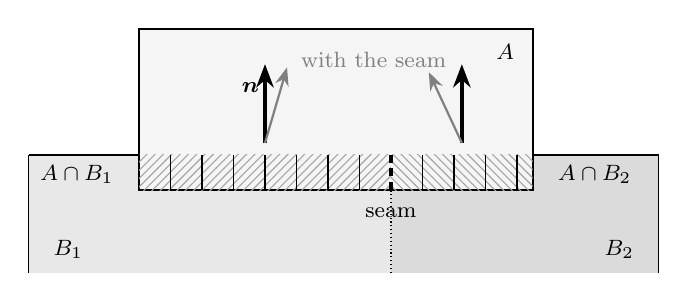
\begin{tikzpicture}[scale=1.0, font=\footnotesize, >=Stealth]
  % Ground pieces B1 and B2.
  \fill[gray!18] (-4,-1.5) rectangle (0.6,0);
  \fill[gray!28] (0.6,-1.5) rectangle (4,0);
  \draw[thick] (-4,0) -- (4,0);
  \draw (-4,-1.5) -- (-4,0) (4,-1.5) -- (4,0);
  \draw[densely dotted] (0.6,-1.5) -- (0.6,-0.45);
  \node at (-3.5,-1.2) {$B_1$};
  \node at (3.5,-1.2) {$B_2$};
  % Body A, flat bottom pressed in by 0.45.
  \fill[gray!8] (-2.6,-0.45) rectangle (2.4,1.6);
  \draw[thick] (-2.6,-0.45) rectangle (2.4,1.6);
  \node at (2.05,1.3) {$A$};
  % Overlaps with each piece.
  \fill[pattern=north east lines, pattern color=gray!70] (-2.6,-0.45) rectangle (0.6,0);
  \fill[pattern=north west lines, pattern color=gray!70] (0.6,-0.45) rectangle (2.4,0);
  % Seam inside the overlap.
  \draw[very thick, densely dashed] (0.6,-0.45) -- (0.6,0);
  \node[anchor=north] at (0.6,-0.55) {seam};
  % Columns of the whole bodies.
  \foreach \xx in {-2.2,-1.8,-1.4,-1.0,-0.6,-0.2,0.2,1.0,1.4,1.8,2.2} {
    \draw[thin] (\xx,-0.45) -- (\xx,0);
  }
  % Normals: with the seam (tilted) and without (law).
  \draw[->, very thick] (-1.0,0.15) -- ++(0,1.0);
  \draw[->, thick, gray] (-1.0,0.15) -- ++(0.28,0.96);
  \draw[->, very thick] (1.5,0.15) -- ++(0,1.0);
  \draw[->, thick, gray] (1.5,0.15) -- ++(-0.42,0.9);
  \node[anchor=east, inner sep=2pt] at (-1.0,0.85) {$\n$};
  \node[gray, anchor=west, inner sep=2pt] at (-0.62,1.2) {with the seam};
  % Labels.
  \node[anchor=west] at (2.6,-0.25) {$A\cap B_2$};
  \node[anchor=east] at (-2.8,-0.25) {$A\cap B_1$};
\end{tikzpicture}

\caption{A body $A$ on a ground $B$ cut into the convex pieces $B_1$ and $B_2$ (section). The
overlap of $A$ with each piece is closed by a seam face (dashed), which enters the volume
integrals of the piece but carries no pressure and does not end a column: the columns (thin
lines) are those of the whole bodies. With the seam, the vector area of the faces of $B_1$ in
the overlap tilts by the ratio of the seam to the contact face; the normal of the distributed
law (arrows) leaves the seam out}
\label{fig:seams}
\end{figure}

\subsection{Deep overlaps}

The vector area $\vect{S}_B$ cancels when the part of $\partial\region$ on $B$ closes on itself
or is empty: a body entirely inside another, or one that pierces another through. Near those
configurations the normal is ill-conditioned, and a law that dropped the pair there would lose
its force at the deepest penetrations. The intersection therefore reports no normal when
$|\vect{S}_B| < 0.1\, V^{2/3}$ (a compact overlap bounded by $B$ on one side has a ratio of
about 2: 1.9 for a half sphere, 2 for the corner of a cube), and the pair then keeps the normal
of its last evaluation, stored in the frame of $B$ as part of the state of the pair: the
direction along which the body came in. A pair that starts that deep takes the outward normal
of the nearest surface face of a convex $B$. Both laws use this fallback.

\subsection{Columns and the exact partition}\label{sup:columns}

The distributed law requires convex shapes (or convex pieces), so that the overlap is convex
and every column is a single segment. A column through a point $\x$ of the contact surface runs
along $\vect{u} = +\n$ from a face of $A$ and along $\vect{u} = -\n$ from a face of $B$, and
ends at the first face of the surface of either body. A face with outward unit normal $\m_f$
and plane $\m_f\cdot\vect{y} = e_f$ ends it only if $\m_f\cdot\vect{u} > 0$, at the distance
$(e_f - \m_f\cdot\x)/(\m_f\cdot\vect{u})$, which is an affine function of $\x$. The column
length is the smallest of these,
\begin{equation}
  \ell(\x) = \min_{f\,:\;\m_f\cdot\vect{u} > 0}\; \frac{e_f - \m_f\cdot\x}{\m_f\cdot\vect{u}} ,
  \label{eq:column}
\end{equation}
over the faces of both shapes that are surface of their bodies. Seams are left out of the
minimum: behind a seam the body continues, so the columns are those of the whole bodies however
they are cut (Fig.~\ref{fig:seams}). Only the faces that can be the first need to be examined:
those that bound the overlap and, for a shape without seams, those within the reach of the
polygon, found with the box tree.

A column carries $K\ell$. When its two ends lie on different bodies, each end carries half
($\gamma = \tfrac12$), so the law is symmetric in $A$ and $B$. When both ends lie on the same
body, which happens when the overlap encloses a body or pierces it, the end that pushes $A$ out
carries it whole ($\gamma = 1$), so that the force stays $K V$ and is continuous through the
enclosure.

On a polygon of $\partial\region$, $\ell$ is the minimum of a few affine functions. The polygon
is split into the convex regions where each face is the one that ends the column, by clipping
it against the lines where two of the affine functions are equal (Fig.~\ref{fig:partition}). On
each region $\ell$ is affine, so the integrals of the elastic pressure and of its moment are
those of a linear function over a polygon and have no quadrature error, whatever the size of
the triangles of the mesh.

\begin{figure}[!htbp]
\centering
% A polygon of the contact surface split by the face where its columns end, and cut where g = 0.
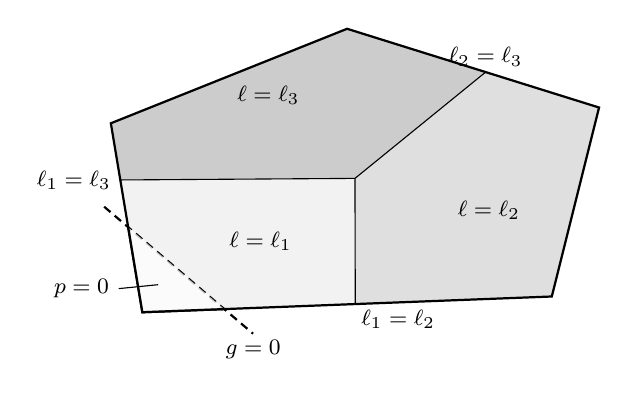
\begin{tikzpicture}[scale=1.0, font=\footnotesize, >=Stealth]
  % Polygon (a face fragment), seen along n.
  \coordinate (v1) at (0,0);
  \coordinate (v2) at (5.2,0.2);
  \coordinate (v3) at (5.8,2.6);
  \coordinate (v4) at (2.6,3.6);
  \coordinate (v5) at (-0.4,2.4);
  % Interior point where the three affine functions are equal, and the points where the
  % dividing lines leave the polygon.
  \coordinate (c) at (2.7,1.7);
  \coordinate (e1) at ($(v1)!0.52!(v2)$);
  \coordinate (e2) at ($(v3)!0.45!(v4)$);
  \coordinate (e3) at ($(v5)!0.3!(v1)$);
  \fill[gray!10] (v1) -- (e1) -- (c) -- (e3) -- cycle;
  \fill[gray!25] (e1) -- (v2) -- (v3) -- (e2) -- (c) -- cycle;
  \fill[gray!40] (c) -- (e2) -- (v4) -- (v5) -- (e3) -- cycle;
  \draw[thick] (v1) -- (v2) -- (v3) -- (v4) -- (v5) -- cycle;
  \draw (c) -- (e1) node[below right, inner sep=2pt] {$\ell_1 = \ell_2$};
  \draw (c) -- (e2) node[above, inner sep=2pt] {$\ell_2 = \ell_3$};
  \draw (c) -- (e3) node[left] {$\ell_1 = \ell_3$};
  \node at (1.5,0.9) {$\ell = \ell_1$};
  \node at (4.4,1.3) {$\ell = \ell_2$};
  \node at (1.6,2.75) {$\ell = \ell_3$};
  % Line g = 0 cutting a corner.
  \coordinate (g1) at ($(v1)!0.2!(v2)$);
  \coordinate (g2) at ($(v1)!0.45!(v5)$);
  \draw[densely dashed, thick] ($(g1)!1.25!(g2)$) -- ($(g1)!-0.3!(g2)$) node[below, inner sep=2pt] {$g = 0$};
  \fill[white, opacity=0.75] (g1) -- (v1) -- (g2) -- cycle;
  \draw[thick] (g1) -- (v1) -- (g2);
  \node[anchor=east] at (-0.3,0.3) {$p = 0$};\draw[thin] (-0.3,0.3) -- (0.2,0.35);
\end{tikzpicture}

\caption{A polygon of the contact surface, seen along $\n$. The column length $\ell$ is the
minimum of the affine functions $\ell_1$, $\ell_2$, $\ell_3$ of the three faces where a column can
end; the polygon is split along the lines where two of them are equal (solid lines), and on each
part $\ell$ is affine. Where the damping factor $\varphi$ changes sign the part is cut again (dashed
line) and the tensile side carries no pressure}
\label{fig:partition}
\end{figure}

\subsection{Damping along the pair normal and the exact clamp}

The rate in the damping factor $\varphi = 1 - h\,\n\cdot\vv$ is measured along the pair normal,
not along the normal of the face, for the following reason. The two ends of the column through
$\x$ are material points of $A$ and of $B$, a distance $\ell$ apart along $\n$. The relative
velocity field is rigid, so the velocities at the two ends differ by $\w\times\ell\n$, which has
no component along $\n$: the quantity $\n\cdot\vv$ is the same all along the column, and it is
the rate at which the column shortens. Sliding along $\n$'s tangent plane and spinning about
$\n$ therefore damp nothing, on any face. Measured along the normal of each face instead, the
slip along any face not perpendicular to $\n$ would count as an approach velocity, which on the
seams of a many-piece bearing is a viscous drag larger than the friction itself.

Without adhesion the pressure cannot be negative. The factor $\varphi$ is affine on the whole
polygon, so where it changes sign the region is cut along the line $\varphi = 0$ and only the
side $\varphi > 0$ is kept (Fig.~\ref{fig:partition}). On what remains, $p$ is the product of
two affine functions, $f = \gamma K\ell$ and $\varphi$. For a triangle of area $A_T$ with
barycentric coordinates $\lambda_k$ and vertex values $f_k$, $\varphi_k$,
\begin{equation}
  \int f\,\varphi\,\lambda_k\,\dd A
  = \frac{A_T}{60}\left(F \Phi + Q + \varphi_k F + f_k \Phi + 2 f_k \varphi_k\right),
  \label{eq:product}
\end{equation}
with $F = \sum_i f_i$, $\Phi = \sum_i \varphi_i$ and $Q = \sum_i f_i \varphi_i$, which follows from
$\int \lambda_i\lambda_j\lambda_k\,\dd A = A_T\,c_{ijk}/60$ with $c_{ijk} = 6$,
$2$ or $1$ for three, two or no equal indices. The three integrals of Eq.~\eqref{eq:product}
give the force of the triangle and its moment exactly. They are also the integrals of the linear
pressure with vertex values
\begin{equation}
  \tilde p_k = \tfrac15\left(\varphi_k F + f_k \Phi + 2 f_k \varphi_k\right) - \tfrac1{20}\left(F \Phi + Q\right),
  \label{eq:equivalent}
\end{equation}
since a linear function satisfies
$\int \tilde p\,\lambda_k\,\dd A = \tfrac{A_T}{12}(\sum_i \tilde p_i + \tilde p_k)$. Each triangle
stores $\tilde p$. The normal force and its moment are thus exact and do not depend on how a
polygon is triangulated; the friction sees the linear equivalent $\tilde p$, which is the exact
pressure whenever $\ell$ or $\varphi$ is constant on the triangle.

\subsection{Normal wrench and the side faces}

The pressure acts along the normal of the face it is on: a triangle of $\partial\region_A$ with
outward normal $\m$ pushes $A$ along $-\m$, one of $\partial\region_B$ along $+\m$. The normal
wrench on $A$ is the sum over the triangles of $\int \tilde p\,\dd A$ times that direction,
applied at $\int \tilde p\,\x\,\dd A / \int \tilde p\,\dd A$. For a flat contact the faces of
$A$ and of $B$ in $\partial\region$ are both perpendicular to $\n$, each carries half, and the
resultant is $K V \varphi(\vect{c})$ at the centre of pressure. On the thin side faces of an
overlap, which are nearly parallel to $\n$, the columns are short and the pressure has no
component along $\n$; it is a small lateral pressure of order $\delta/L$ of the normal load for
a contact of depth $\delta$ and width $L$, and it carries friction, so that the ratio of
friction to normal load is $\mu\,(1 + O(\delta/L))$: a systematic bias against pure Coulomb
friction of $10^{-3}$ to $10^{-2}$ at the depths of the battery, below the thresholds at which
the results are read. This is the difference between a pressure on the faces, which is what the
law applies, and a traction along $\n$ per unit of projected area, which is what a strict
Winkler bed would apply; the two agree to first order in the depth.

\subsection{Friction: special cases and what is exact}

Two cases fall outside the instantaneous centre of Eq.~6 of the paper. When the triangle does
not rotate in its plane ($\omega_m = 0$) the slip is uniform, and the friction is
$\mu\int p\,\dd A$ against it, applied at the centre of pressure of the triangle. When the
centre is far, the three signed terms are large and nearly cancel, so the same uniform-slip
formula is used whenever $|\omega_m|\sqrt{2A_T} \le 10^{-3}|\vv_{t0}|$, with the direction of
the slip taken at the centre of pressure. At the switch the force changes by a relative
$10^{-6}$ and the moment of one triangle jumps by up to about $3\times10^{-4}$ of
$\mu\int p\,\dd A$ times its size: far below every other error of the paper, but a
discontinuity.

The friction is exact for the pressure $\tilde p$ of each flat triangle. It is not exact where
$\tilde p$ is not the true pressure, that is, where both $\ell$ and $\varphi$ vary over a
triangle; on a faceted body spinning in a faceted seat this leaves a residual torque of the
nature of a rolling resistance, of order $h\,\omega\,b^2/(12\,\mu\,r)$ of the friction torque
for facets of width $b$ at a radius $r$, which decreases with the square of the facet width. A
face that is a seam only in part counts as surface.

The check of the closed form (\code{paper/checks/check\_polar\_moments.py}) re-implements the
formulas of the paper's Section~3.4 and Appendix~A as printed and compares them with
quadrature that does not use them, for $\q$ outside, inside, on an edge and at a vertex of the
triangle; the moments agree to $10^{-14}$ with a Gauss--Legendre rule where the integrand is
analytic and to the accuracy of a midpoint rule ($10^{-5}$) elsewhere.
% The numbers of this paragraph are those the script prints; they are not battery results.

\subsection{Gonthier's law: stick--slip and the variant of the 2018 thesis}

The force $\Fn = K V(1 - h\,v_n(\vect{c}))$ is exact volumetric damping, because $v_n$ is an
affine function of position and its integral over $\region$ is $V$ times its value at the
centroid. $\Fn$ is clamped at zero, and the rolling torque is not applied while the clamp is
active, since the pressure whose moment it is has vanished. Between pure sliding and pure
spinning the friction satisfies
$(|\vect{f}_t|/\mu\Fn)^2 + (|\vect{M}_s|/\mu\Fn r_g)^2 = 1$.

Stick--slip follows the thesis \cite{Gonthier2007thesis} in its structure: a sticking function
$s = \exp(-v_\mathrm{avg}^2/v_s^2)$ blends a bristle force and a torsional bristle torque (the
latter with stiffness and damping multiplied by $r_g^2$) with the sliding values. As in the
thesis, the sliding values are shares of one friction budget: the force takes the fraction
$C_{v,s} = s + (1-s)\,C_v$ of it and the spinning torque $C_{\omega,s} = s + (1-s)\,C_\omega$,
with $C_v = |\vv_t|/\max(v_\mathrm{avg}, v_\varepsilon)$,
$C_\omega = r_g|\omega_n|/\max(v_\mathrm{avg}, v_\varepsilon)$ and the floor
$v_\varepsilon = v_s/100$ that avoids the division by zero at rest; the sliding targets are
$\mu_d F_n C_{v,s}$ and $\mu_d r_g F_n C_{\omega,s}$.

The implementation departs from the thesis in four points, none of which changes the sliding or
the spinning law: the bristle is a spring--damper on the deflection blended with the sliding
force by $s$, the regularization of Dopico et al.~\cite{Dopico2011}, instead of a bristle state
integrated with its own differential equation; the dwell-time dependence of the static friction
is not implemented; the normal is the vector-area normal; and $V$ and $\tens{J}$ are exact for
the meshes, where the thesis approximates them with voxels.

The law \law{gonthier-thesis} keeps the friction of the second author's thesis
\cite{Vilela2018}. Its sliding force ignores the spin, its spinning torque is
$\vect{M}_s = -\mu_\mathrm{spin}\,(\Fn/V)\,\tens{J}\,\omega_n\n$, which is the expression of
the 2005 paper \cite{Gonthier2005} read with a constant coefficient and is therefore viscous
($\mu_\mathrm{spin}$ carries s/m), and its bristle is a spring between the centroid of the
overlap and an anchor fixed in $B$. The centroid of the overlap is not a material point: when a
body on a flat contact of width $L$ and depth $\delta$ rocks by an angle $\theta$, the centroid
moves by $L^2\theta/(12\,\delta)$: 0.22\,mm per microradian for $L = 0.4$\,m and
$\delta = 60$\,\textmu m, values of the battery, so 2\,mm for a rocking of 10\,\textmu rad. The
anchored bristle therefore stretches with nothing sliding. Gonthier's own bristle integrates
the relative velocity at the contact, a material quantity, and that is what \law{gonthier}
does.

\subsection{Stiction}

\paragraph{Transition.} The speed $u$ that drives the weight $s = \exp(-u^2/v_s^2)$ is
Gonthier's $v_\mathrm{avg}$ in \law{gonthier}; in \law{distributed} it is its counterpart for
the pressure distribution, $u^2 = |\vv_t(\vect{c}_p)|^2 + \rho^2\omega_n^2$, with $\vect{c}_p$
the centre of the normal load and $\rho$ the radius of gyration of the pressure about it.

\paragraph{Deflection.} The deflection is the slip of the material point of $A$ that is at the
friction point, relative to $B$, accumulated from one evaluation to the next and kept in the
frame of $B$; the torsional deflection accumulates the rotation of $A$ relative to $B$ about
$\n$. The friction point is the centroid of the overlap in \law{gonthier} and the centre of the
normal load in \law{distributed}. Because what is accumulated is the motion of material points
between two evaluations, rolling without slipping loads no bristle, a displacement of the
friction point caused by a change of shape of the overlap loads none either, the state is
objective, and the accumulated slip does not depend on the time step. The state of a pair is
the deflection, the twist, the relative pose at the last evaluation and the last pair normal.

\paragraph{Stiffness proportional to the load.} With $k = \mu_s|\Fn|/d$ and $c = k\tau$ (the
torsional bristle has $k\rho^2$ and $c\rho^2$, $r_g^2$ in \law{gonthier}), every contact
reaches its static limit after the same displacement whatever its load, as in Gonthier's
bristle, whose stiffness is $\mu_s/\delta_z$ times the normal force \cite{Gonthier2007thesis}.
For a body resting on its contact under its own weight the bristle has $\omega^2 = \mu_s g/d$
whatever the mass, and $\tau$ gives it a damping ratio $\tau\omega/2 \approx 0.55$ for
$\mu_s = 0.5$. The sensitivity of the results to $d$ and $\tau$ was not swept.

\paragraph{Limits.} The spring force never exceeds the static limit; when it would, the
deflection is scaled back onto the limit, which is the slip of the bristle. The damper alone
would reach the static limit at the creep velocity $d/\tau = 20$\,mm/s and brake a body that
must slide like a viscous drag, so the total stick force, spring plus damper, is capped at the
limit as well. In \law{gonthier} the limits of the bristle force and of the torsional bristle are
$\mu_s\Fn$ and $\mu_s\Fn r_g$ times the shares of Gonthier's thesis, which both tend to 1 at
stick. The static limit of \law{gonthier}, as published and as coded, is therefore a box: a
patch at rest can hold a force of $\mu_s\Fn$ and a torque of $\mu_s\Fn r_g$ at once, up to
$\sqrt2$ times what its friction ellipse allows. In \law{distributed} the translational and the
torsional bristle share the friction through the limit surface of the patch, approximated by
the ellipse of Howe and Cutkosky \cite{Howe1996},
\begin{equation}
  \left(\frac{|\vect{f}_\mathrm{stick}|}{\mu_s\Fn}\right)^2
  + \left(\frac{|M_\mathrm{stick}|}{T_\mathrm{max}}\right)^2 \le 1 ,
  \qquad T_\mathrm{max} = \mu_s\int p\,|\x - \vect{c}_p|\,\dd A ,
  \label{eq:ellipse}
\end{equation}
where $T_\mathrm{max}$, the static spinning capacity of the pressure distribution, is the
pressure-weighted polar moment $\sum(p_q D + \nabla p\cdot\vect{R})$ over the triangles, with
the centre at $\vect{c}_p$. Limiting each bristle on its own lets a patch cut into pieces, each
of which sees a twist of the body as slip plus twist, hold more than the whole patch. The stick
acts in the plane of the pair normal, at the centre of the normal load and with the capacity of
the normal load, so that it adds up over the pieces of a body. The state remains one per pair
of pieces; a single state per pair of bodies would not do, because one body pair can touch on
several planes whose normal loads cancel in the sum and define no tangent plane.

\subsection{Properties of the distributed law}

None of the following is a result of the battery. Those marked as not asserted are not covered
by a test of the library.
\begin{itemize}
\item \emph{Reduction to Gonthier's law.} For a flat contact the normal force is
  $K V(1 - h\,v_n(\vect{c}))$ at the centre of pressure, with Gonthier's rolling resistance.
\item \emph{Closed cycle and fast paths.} The elastic force of a sphere in a faceted bowl does
  no work over a closed cycle, and the fast paths give the same overlap and forces as the plain
  ones.
\item \emph{Symmetry (not asserted by a test).} Exchanging $A$ and $B$ gives the opposite wrench
  exactly for single convex pieces and only approximately for compounds, because the pair
  normal is taken from the non-seam faces of $B$.
\item \emph{Independence of the triangulation} for the normal wrench (exact partition and exact
  clamp), and \emph{independence of the decomposition}: a box sliding or spinning on a slab
  receives the same wrench on a slab cut into pieces as on the whole slab, to a relative
  difference below $10^{-9}$. The scenarios \scn{pieces} test the same property dynamically.
\item \emph{Continuity in the pose (by construction, not asserted by a test).} The surface of
  the overlap, the column lengths and the partition vary continuously with the pose, so the
  wrench does; no face switches on or off as a sample point crosses a surface.
\item \emph{Force at deep overlaps.} A body enclosed in another, or through it, keeps a force
  $K V$ along the last normal.
\end{itemize}
The elastic force is conservative while the normal of a pair is fixed and is not exactly so
where that normal turns with the overlap (a relative work of $10^{-4}$ over a closed cycle at
the rim of a faceted bowl; Elandt et al.~\cite{Elandt2019} note the same of elastic-foundation
models in general). The differentiability of the wrench was not analysed.

\subsection{Baselines: departures from the publications}

The baselines live in the same library, run on every engine like the two laws, receive the same
$K$, $h$ and $\mu$, and are subject to the same step bounds (Section~\ref{sup:steps}).

\paragraph{Friction quadratures.} The two variants of \law{distributed} change only the
friction: the geometry, the pressure and its clamp, the normal wrench and the stiction are the
same code. The vertex rule evaluates the friction $-\mu\,p_i\,\vv_{t,i}/|\vv_{t,i}|$ at the
three vertices of each triangle (zero at a vertex that does not slip) and interpolates it
linearly, which gives the force $\tfrac{A_T}{3}\sum_i\vect{f}_i$ and the moment of a linear
field. The equations of Hasegawa and Sato \cite{Hasegawa2004} are used as we understood them
from a reading of the paper made for the review of the literature; the paper was not accessible
to us again, so the rule was not re-checked against its Eqs.~13 to~16, and it should be read as
the vertex interpolation that the paper describes and not as a verified transcription. Their
model, which projects the triangles on one contact plane, is not reproduced, only its friction
quadrature.

\paragraph{The per-face foundation.} In \law{pcm} both bodies carry springs, each with half the
stiffness, so that a flat contact carries $K V$ as the other laws do; the force of a spring is
never negative, and the friction is a continuous function of the slip velocity with the
transition velocity $v_s$ of the other laws. The law has no stiction and keeps no state, as its
sources have none (Simbody's documentation says that the model cannot represent stiction): a
body loaded below its friction limit creeps. The implementation departs from the publications
\cite{Hippmann2004,Hippmann2024,Sherman2011,SimbodyEFF} in four points, and the first two
favour the baseline. (i) The elements are the triangles of the exact contact surface, the part
of each face inside the other body, and not the whole faces whose centroid is inside: with the
two triangles per face of the battery's grounds the published sampling would leave them without
contact, and the publications ask for a fine mesh instead. What remains of the published
discretization is one sample of depth, velocity and slip per element. (ii) The penetration is
measured to the nearest point of the other surface, as in Simbody, and not along the normal of
the element. (iii) The damping is the product form $\tfrac12 K A_T\,x\,(1 + h\,\dot x)$; the
polygonal contact model has a constant areal damping. (iv) There is no viscous friction term.

\subsection{Cost of a pair and of the laws}

The cost of one pair is that of clipping the faces of each shape that lie in the candidate
region against the other shape; it grows with the number of faces in the region and not with the
size of the meshes, and it does not depend on the depth of the overlap. Pairs are independent
and are evaluated in parallel, with one scratch workspace per thread so that no memory is
allocated after the first step, and their wrenches are accumulated in a fixed order so that the
result does not depend on the number of threads.

The geometry is shared by the two laws. Gonthier's law adds a constant amount of arithmetic per
pair. The distributed law adds, per polygon of the contact surface, the search for the faces
where its columns can end, the partition, and per resulting triangle the closed forms of
the product integral and of the polar moments; its cost grows with the number of faces in
contact. Curved bodies meshed with many small faces are the expensive case: the cap of a
64-segment sphere on a plane has tens of triangles in contact, a box on a plane has two. The
measured costs are in Section~\ref{sup:cost}.

\section{Stability of the explicit step and step bounds}\label{sup:steps}

% The paper cites these subsections by number (S2.1 to S2.4): keep their order.

\subsection{Coupling with the engines}

The contact model knows nothing of the engine: bodies are indices, and the friction state is
passed in and out so that each engine can keep it where its stepping scheme requires. The
backends are thin: each one builds the engine's model of a scenario, and at every step reads the
state, evaluates the contact model, applies the wrenches as external forces and advances. The
friction state advances once per step, from the same evaluation. The contact models of the
engines themselves are switched off for the methods of the library.
\begin{itemize}
\item \emph{Drake} (version 1.58). The bodies are free bodies of a discrete
  \code{MultibodyPlant} without contact geometry. A system connected to the plant outputs the
  wrenches as externally applied spatial forces and holds the friction state as discrete state
  with the period of the plant, and serves to the plant the evaluation made at the start of the
  step, so that the forces act on the state they were computed from.
\item \emph{Project Chrono} (version 10.0). The wrenches are accumulated on the bodies at their
  centres of mass before each step of the linearized implicit Euler time stepper, for which an
  external load is a constant.
\item \emph{MuJoCo} (version 4.0). Bodies have free joints; the wrenches are written as applied
  Cartesian forces and the step is taken with the \code{implicitfast} integrator, whose implicit
  terms do not include applied forces.
\end{itemize}
Each backend also passes its step and the inverse inertias of the bodies to the contact model,
which is what the bounds of Section~\ref{sup:bounds} need; the engines store the state of a
pair as 26 numbers. For a free body under an applied force the three steppers are the same
first-order scheme, the semi-implicit Euler step: the velocity is advanced with the force of
the start of the step and the position with the new velocity. They differ in how they integrate
rotation and gyroscopic terms.

\subsection{Stability condition}

The step is $\vv^+ = \vv + \dt\,M^{-1}\vect{f}(\x,\vv)$, $\x^+ = \x + \dt\,\vv^+$. For a spring
$k$ and a damper $c$ acting on an inverse mass $w$, with $\alpha = k\,w\,\dt^2$ and
$\beta = c\,w\,\dt$, one step maps $(x, \dt\,v)$ with the matrix
$\bigl(\begin{smallmatrix} 1-\alpha & 1-\beta\\ -\alpha & 1-\beta\end{smallmatrix}\bigr)$, whose characteristic
polynomial is $\lambda^2 - (2-\alpha-\beta)\lambda + (1-\beta)$. By the Jury conditions the scheme is stable
if and only if $0 < \alpha$, $\beta < 2$ and $\alpha + 2\beta < 4$ (at $\alpha = 0$ it is only marginally stable), that is,
\begin{equation}
  k\,w\,\dt^2 + 2\,c\,w\,\dt < 4 \quad\text{and}\quad c\,w\,\dt < 2 .
  \label{eq:sup-stability}
\end{equation}
When several contacts act on a body their contributions add. Four mechanisms of the laws enter
this condition, and three of them are proportional to the load: the stick spring and damper;
the normal damper, $c = h\,K V$; and the sliding friction across the stick--slip transition,
which is a damper of up to $0.86\,\mu\Fn/v_s$. For a body of mass $m$ under a contact load of
$N$ times its weight, with $h = 5$\,s/m, $\mu = 0.5$ and $\dt = 1$\,ms, the stick has
$\alpha + 2\beta = 0.54\,N$, so the default bristle is stable up to a load of about seven times
the weight; the normal damper has $\beta = 0.049\,N$ and the transition $\beta = 0.17\,N$. A
body under its own weight is far from all three limits. A block at the bottom of a tall stack,
or a light body under a heavy one, is not.

The fourth mechanism is the normal stiffness, which is the model's and is not touched, since
changing it would change the statics. For a flat contact of area $A_c$ between a body of mass
$m$ and the ground it needs $K A_c\,\dt^2/m < 4$; for a body held between two such contacts the
two stiffnesses add, $\sum w = 2/m$, and with the dampers at their bounds the condition
$K A_c\,\dt^2\sum w < 2$ gives $\dt < \sqrt{m/(K A_c)}$. The stiffnesses of the battery were
chosen so that the base step of 1\,ms satisfies it, with the two exceptions that are there to
show the limit.

\subsection{Bounds on the terms proportional to the load}\label{sup:bounds}

Let $\Lambda = \sum|\Fn|\,w$ be the \emph{load acceleration} of a body, the sum over its
contacts of the normal force times the inverse mass that the contact sees. With $\Lambda$ the
sum of the load accelerations of the two bodies of a pair, each pair applies
\begin{equation}
  k \le \frac{|\Fn|}{\Lambda\,\dt^2}, \qquad c \le \frac{|\Fn|}{\Lambda\,\dt}, \qquad
  h \le \frac{1}{\Lambda\,\dt}, \qquad v_s \ge \mu\,\Lambda\,\dt ,
  \label{eq:bounds}
\end{equation}
and the torsional bristle the same with the inverse inertia about the normal, so that each
mechanism satisfies $\sum k\,w\,\dt^2\le1$ and $\sum c\,w\,\dt\le1$ over the contacts of a body,
which keeps Eq.~\eqref{eq:sup-stability} with margin when two mechanisms act on one body. In
words: a stick spring cannot bring the pair back in less than a step, a damper cannot take more
than the relative velocity of a step, and the stick--slip transition cannot be narrower than
the change of velocity that friction causes in a step. The load acceleration counts the lever
arm of each contact and, for the normal damper, the rocking that the damping of the foundation
resists; it is at least the pair's own. $\Lambda$ is taken from the previous evaluation and
kept in the state of the pair. The bounds are per unit of load, so they do not depend on how a
contact is cut into pieces, and there is no sub-stepping. The baselines of the library are
subject to the same bounds.

\subsection{What the bounds change}

Below the threshold of Eq.~\eqref{eq:bounds} nothing changes: a body under its own weight at
1\,ms receives the same wrench to the last bit with and without the bounds, which a test of the
library asserts. Above it, the parameters that the user gave are no longer the ones applied: the
pre-sliding displacement grows from $d$ to $\mu\Lambda\,\dt^2$, the stick--slip transition widens
to $\mu\Lambda\,\dt$, and the damping factor falls below $h$, all as functions of the step and of
the load; the dampers that a light body carries are bounded by its mass over the step, so a
heavy body resting on a light one is damped less than the model prescribes. What is benchmarked
there is the law regularized by the step, and its results converge to the model's only as the
step is reduced. The battery did not record in which runs the bounds were active; from the
loads, they are in \scn{tower}, \scn{massratio} and \scn{stack} at the base step and are not in
the scenarios with one body under its own weight.

\clearpage
\section{Native contact models: configurations and results of our configurations}\label{sup:natives}

% The paper cites these subsections by number (S3.1 to S3.6): keep their order.

Everything in this section is a result of the configurations described in
Section~\ref{sup:native-config}. They are ours: none was reviewed by the developers of an
engine. The paper draws from the native runs only what follows from a property of a model
family; the results below go beyond that, several are unexplained, and none should be read as
the performance of an engine in expert hands.

\subsection{Configurations}\label{sup:native-config}

Each native model has one configuration, the same for every scenario, built from the engine's
documentation and written down with its sources in the specification of the repository
(\code{docs/scenarios.md}, Section~3). The names are used as written here throughout;
``point-contact models'' means the five other than Drake hydroelastic, which are a penalty
model with one point per pair (Drake point), a penalty model on a manifold (Chrono SMC), a
complementarity solver (Chrono NSC) and soft constraints (the two of MuJoCo). Every native run
has a wall-clock limit of one hour in the base variant and ten minutes in the series (half an
hour for the methods of the library).

The scenario gives every method the same $K$, $h$ and $\mu$. Models whose stiffness belongs to
a contact point (N/m) have no areal stiffness on which to map $K$; they use a reference area
$A_\mathrm{ref}$, one sixth of the surface of a solid (the face of a cube), so that
$K A_\mathrm{ref}$ is the stiffness of a foundation $K$ under a face of that size. This sets
the scale and is exact only when the contact is a face of that area.

\paragraph{Drake, hydroelastic} (the default native model of Drake in this paper)
\cite{DrakeHydroGuide,DrakeHydroParams}. Planar grounds are compliant half-spaces and other
grounds are compliant tetrahedral meshes, with hydroelastic modulus $E = K H$, $H$ being the
depth of the pressure field, so that the pressure is $K$ times the depth: with a rigid
counterpart this is a Winkler foundation of the same $K$ evaluated on the rigid surface. Bodies
are rigid unless they touch another rigid body; the contact graph is two-coloured from the
grounds. A rigid body that touches a half-space has its surface refined until no edge exceeds
one eighth of its largest side, because Drake turns each polygon of the contact surface into one
contact point and the guide warns that the refinement of a contact with a half-space is that of
the other geometry; an unrefined box stands on two points. Dissipation is of Hunt--Crossley
type with coefficient $h$, with the discrete approximation that keeps that form (``lagged''),
and the friction coefficients of the geometries are solved so that Drake's combination rule
gives the $\mu$ of each pair.

\paragraph{Drake, point} \cite{DrakePointContact}. Compliant point contact in the same plant
and solver, between analytic primitives or convex pieces, with point stiffness $K A_\mathrm{ref}$
per geometry (Drake combines two geometries in series) and dissipation $h$. A box carries a
small sphere at each corner, the device of Drake's own box models \cite{DrakeFoamBrick}, since
one point per pair cannot hold a face.

\paragraph{Chrono, SMC} (the default for Chrono) \cite{ChronoCollisions,ChronoSMCSource}.
Analytic primitives where the scenario has them and convex pieces otherwise. Hooke's law with
explicit coefficients: normal and tangential stiffness $K A_\mathrm{ref}/4$ per contact point
(a face contact has a manifold of four), and a normal damping that is the Hunt--Crossley term
linearized at the static penetration under the body's weight. In the version used, the
Jacobians of the contact force are disabled in the source and the tangential displacement is
that of one step, so the model is explicit and has no stiction memory; the backend sub-steps so
that the contact oscillation is resolved with at least 60 steps, and uses the stiffest tangential
damping that an explicit step integrates, which bounds the creep of a held body but does not
remove it.

\paragraph{Chrono, NSC} \cite{ChronoSystem}. The complementarity formulation for rigid contact,
with the same shapes, the pair's $\mu$ and zero restitution; $K$ and $h$ do not enter. Solved
with the Barzilai--Borwein method \cite{Barzilai1988}, which the manual recommends when
accuracy matters.

\paragraph{MuJoCo, soft} (the default for MuJoCo) \cite{MuJoCoDocs,MuJoCoModeling}. MuJoCo's
contact model with the values that its manual recommends for new models: analytic primitives
or convex pieces, elliptic friction cones, a tight solver tolerance, a few no-slip iterations
and the \code{implicitfast} integrator. The stiffness of the constraint is set so that the
static force of a flat contact is $K A_\mathrm{ref}$ times the penetration; only the statics
are a spring's, because the constraint also removes a fixed share of the load that presses the
bodies together. Damping is critical: MuJoCo's damper is linear and cannot follow the dependence
of the Hunt--Crossley restitution on the impact speed. Each contact has torsional friction with
the coefficient of a disk of its patch area under uniform pressure.

\paragraph{MuJoCo, default.} The same geometry with MuJoCo's own default parameters and
options: what a user obtains without changing anything. $K$ and $h$ do not enter.

\subsection{Revisions and known asymmetries}

The configurations were not fixed blind: after the first complete run of the development
scenarios several options were revised with the errors of the battery in view. The revisions
were the refinement of rigid surfaces to one eighth of the largest side for Drake's
hydroelastic contact (\scn{block} went from 13 to 1.4\,\%), the corner spheres of boxes for
Drake's point contact (\scn{block} from 98 to 0.1\,\%), the solver tolerance and the reference
area for MuJoCo (\scn{stack} from 33 to 0.16\,\%) and the choice of the Barzilai--Borwein solver
for Chrono NSC. Each revision was a setting applied to every scenario and was chosen from a
sweep over all of them, never per scenario; they are nonetheless iterations on the scores of
the development set, fewer than those of the laws, recorded in the history of the repository
(\code{docs/history.md}, entries of 11 November 2026). % The four figures are those of that history, single runs on the development scenarios.

Drake's point contact gives a box a small sphere at each corner and
gives a cylinder or a disk nothing: its flat face touches the ground at one point, so the errors
and the runs without a stop time of that model on \scn{disk}, \scn{contensou} and \scn{cone} are
in part a consequence of our configuration and not of the model. Chrono SMC is sub-stepped by the
backend (between 1 and 15 sub-steps per step of the battery), so its step is not the step of the
other methods, in the convergence series and in the costs. The reference area $A_\mathrm{ref}$ is
a scale: for bodies that are not cubes (the plates of \scn{offset} and \scn{tower}, the disk) the
point stiffness of a native model differs from that of the foundation under the face in contact by
factors of 2 to 3. The static penetration of each native model was not compared with the
foundation's scenario by scenario. MuJoCo's recommended configuration misses \scn{block}, the
simplest scenario, by \result{err/block/soft} (\result{pertrange/block/soft/range} over the
perturbed starts); a configuration reviewed by a user of that engine would probably not, and the
result should not be read as representative of expert use.

\subsection{Results by class}

The errors are in the tables of the paper (Tables~3 to~5) and in Section~\ref{sup:errors}.

\emph{Class A.} On the seven scenarios of a body sliding or rolling on one plane, Drake point
and Chrono NSC are as accurate as the two laws or more: in
\result{within/oneplane/dpoint+nsc/0.4} of them the errors of both models are below 0.4\,\%,
though Drake point misses \scn{vgroove} by \result{err/vgroove/dpoint}. MuJoCo soft has
\result{err/block/soft}, \result{err/twoblocks/soft} and \result{err/billiard/soft} in
\scn{block}, \scn{twoblocks} and \scn{billiard}, and MuJoCo default \result{err/push/mjdefault}
and \result{err/twoblocks/mjdefault} in \scn{push} and \scn{twoblocks}. Chrono SMC, which has
no stick memory in the version used, creeps in \scn{push} and \scn{wedge}
(\result{err/push/smc}, \result{err/wedge/smc}). In \scn{bowl} and \scn{trough} the native
models lose between \result{err/bowl/smc} and \result{err/trough/soft} of the amplitude. In
\scn{turntable} Drake point keeps the orbit, with \result{err/turntable/dpoint} and
\result{pertrange/turntable/dpoint/range} over the perturbations; the base run of Chrono NSC
(\result{err/turntable/nsc}) is the best of its perturbed starts
(\result{pertrange/turntable/nsc/range}, median \result{pertrange/turntable/nsc/median}). In
\scn{journal}, Drake hydroelastic and MuJoCo soft are within 5\,\% (\result{err/journal/hydro},
\result{err/journal/soft}; \result{pertrange/journal/soft/range} when perturbed), and Drake
point and Chrono's two models are between \result{err/journal/smc} and
\result{err/journal/nsc}. On the cut ground Chrono's models depend on the cut
(\result{err/pieces64/smc}, and \result{err/pieces2/nsc} for NSC already on two pieces). In
\scn{wedge}, Chrono NSC, MuJoCo soft and Drake point hold the block that must hold. In
\scn{oblique} Chrono SMC and Drake point, on a sphere, are within 0.6\,\%. Chrono NSC and MuJoCo
soft hold \scn{tower} and \scn{massratio} within 1\,\%; Drake hydroelastic holds \scn{massratio}
and did not finish \scn{tower}; Drake point, which uses the same solver, loses both
(\result{err/massratio/dpoint} and \result{err/tower/dpoint}), so being implicit in the contact
force is not sufficient. In \scn{energy} every native model but Chrono SMC has an error above
20\,\% (Drake point \result{err/energy/dpoint}).

\emph{Class B.} Drake point, Chrono NSC and the two MuJoCo models are each outside the band in
\result{band/dpoint/outside} of the five scenarios; Chrono SMC is outside in
\result{band/smc/outside} and has no stop time in \result{band/smc/none}
(Table~\ref{tab:band}). Their errors against the nominal value go from \result{err/ring/smc}
(Chrono SMC in \scn{ring}, below the \result{err/cone/hydro} of Drake hydroelastic in
\scn{cone}) to \result{err/bearing/nsc}. Drake hydroelastic is inside the band in
\result{band/hydro/inside} scenarios and undetermined in the others, with \result{err/disk/hydro}
in \scn{disk}.

\emph{Class C.} Drake hydroelastic is within 5\,\% in \result{pass/C/hydro/5}; \scn{tip} ends
without a value with every point-contact model, as designed: a box on stiff points tips at the
rigid angle, which the ramp of the scenario never reaches.

\emph{Step, mesh and stiffness.} Drake hydroelastic is the method whose error depends most on
the step: it converges in \result{convn/dt/hydro/converging} series, and its errors at 1\,ms in
the rolling and impact scenarios are step errors. It holds \scn{massratio} at every step at
which it finished, as do Chrono NSC and the two MuJoCo models. Chrono SMC is sub-stepped by the
backend, so its series is not one of the step of the battery. With $K\times10$ the errors of
Drake hydroelastic on class A fall in \result{stiffn/hydro/better} of \result{stiffn/hydro/n}
scenarios, and on the flat \scn{disk} its error does not rise (\result{err/disk/hydro/stiff}).

\subsection{Scatter under perturbation}\label{sup:scatter}

Over the eight perturbations of the initial velocities (1\,mm/s and 0.01\,rad/s, from a seeded
generator), the range of the error relative to its median has a median over the scenarios of
\result{pert/hydro} for Drake hydroelastic and \result{pert/soft} for MuJoCo soft, and of
\result{pert/dpoint}, \result{pert/nsc} and \result{pert/smc} for Drake point, Chrono NSC and
Chrono SMC (for the two laws, \result{pert/gonthier} and \result{pert/distributed}). The base
errors are therefore representative of nearby initial conditions for Drake hydroelastic and for
MuJoCo soft, and less so for Drake point and the two Chrono models.
Table~\ref{tab:perturbations} lists the cells of classes A and B in which the perturbed runs of
a native model differ by more than a factor of 2 or lose a run: for those, the base value is
one draw and the median is the better summary. Chrono NSC in \scn{disk} has
\result{err/disk/nsc} in the base run and \result{pertrange/disk/nsc/range} over the
perturbations (median \result{pertrange/disk/nsc/median}).

\begin{table}[!htbp]
\caption{Native models whose error scatters over the eight perturbed starts (classes A and B):
error [\%] of the base run, median and range of the perturbed runs that have a value, and number
of perturbed runs without one}
\label{tab:perturbations}
\generatedtable{perturbations}
\end{table}

\subsection{Unexplained results}

The following results of our configurations have no explanation, and any of them may be an
effect of the configuration. Drake hydroelastic: \scn{hole} (\result{err/hole/hydro}),
\scn{corner} (\result{err/corner/hydro}) and \scn{stack} (\result{err/stack/hydro}), none of
which falls with the step; \scn{tower} and the smallest steps of \scn{stack} and
\scn{massratio} reach the time limit. Chrono NSC: \scn{oblique} and most of \scn{restitution}
end without a rebound value (the model was given zero restitution, so it was not expected to
meet the rebounds, but why some are not produced at all was not traced), \scn{edge} has
\result{err/edge/nsc}, and its mesh variants on \scn{disk} and \scn{turntable}
(\result{err/disk/nsc/mesh32} and \result{err/turntable/nsc/mesh32} at 32 segments,
\result{err/disk/nsc/mesh128} and \result{err/turntable/nsc/mesh128} at 128) differ from its
base runs (\result{err/disk/nsc}, \result{err/turntable/nsc}) although its shapes are analytic
primitives; the scatter of the model over nearby starts is of that size, and what else differs
between those runs was not traced. MuJoCo default: \scn{edge} (\result{err/edge/mjdefault}).
The runs of \scn{disk} and \scn{contensou} with Chrono SMC and Drake point, and of \scn{cone}
with the latter, end without a stop time: in the diagnostic runs of Chrono SMC the spinning
body wobbled on its rim and kept a spin above the 1\,\% that defines the stop; Drake's runs
were not traced, and its disk stands on one point by our configuration.

\subsection{A choice of model by situation, as configured}

Table~\ref{tab:decision-natives} adds to the table of the paper's discussion what the runs of
our configurations show about particular native models.

\begin{table}[!htbp]
\caption{Native models by situation, as far as our configurations show (classes A and B, base
variant)}
\label{tab:decision-natives}
\footnotesize
\begin{tabular}{@{}p{0.27\linewidth}p{0.27\linewidth}p{0.40\linewidth}@{}}
\toprule
Situation & Native models that did well & Evidence \\
\midrule
A rigid body sliding or rolling on one plane; sphere and cylinder contacts &
  Drake point, Chrono NSC &
  \scn{block}, \scn{sphere}, \scn{cylinder}, \scn{twoblocks}: Drake point
  \result{err/block/dpoint}, \result{err/sphere/dpoint}, \result{err/cylinder/dpoint},
  \result{err/twoblocks/dpoint}; \law{distributed} \result{err/block/distributed},
  \result{err/sphere/distributed}, \result{err/cylinder/distributed},
  \result{err/twoblocks/distributed} \\
A flat face that spins, or slides and spins &
  Drake hydroelastic &
  \scn{disk}: \result{err/disk/hydro}; \law{distributed} \result{err/disk/distributed};
  point-contact models outside the band or scattered (Tables~\ref{tab:band}
  and~\ref{tab:perturbations}) \\
Curved conforming contact &
  Drake hydroelastic &
  \scn{bearing} at 128 segments: \result{err/bearing/hydro/mesh128}; \law{pcm}
  \result{err/bearing/pcm/mesh128}, \law{distributed} \result{err/bearing/distributed/mesh128} \\
A body held by friction near its limit &
  Chrono NSC, MuJoCo soft, Drake point &
  \scn{wedge}: \result{err/wedge/nsc}, \result{err/wedge/soft}, \result{err/wedge/dpoint};
  Chrono SMC \result{err/wedge/smc} \\
Stiff contacts on light bodies, large mass ratios, tall stacks at large steps &
  Chrono NSC, MuJoCo soft; Drake hydroelastic where its cost allows. Not every implicit solver &
  \scn{massratio} at 1\,ms: Chrono NSC, MuJoCo soft and Drake hydroelastic within
  \result{err/massratio/soft}; Drake point \result{err/massratio/dpoint}, and
  \result{err/tower/dpoint} in \scn{tower} \\
Long rolling &
  Drake point &
  \scn{turntable}: \result{err/turntable/dpoint} (\result{pertrange/turntable/dpoint/range}
  perturbed); the laws \result{err/turntable/distributed} \\
\botrule
\end{tabular}
\end{table}

\clearpage
\section{Complete tables and figures}\label{sup:results}

% The paper cites these subsections by number (S4.1 to S4.8): keep their order.

All tables and figures of this section are generated from the result files of the repository
(\code{results/battery.csv}, \code{results/terms.csv}, \code{results/stats.json},
\code{results/timing.csv}) by the same script as those of the paper
(\code{tools/paper\_results.py}). The methods of the library are shown by their runs on Chrono.
Abbreviations: Gon (\law{gonthier}), G18 (\law{gonthier-thesis}), Dis (\law{distributed}), Dis-v
and Dis-1 (its vertex and one-point friction rules), PCM; Dr-h and Dr-p (Drake hydroelastic and
point), Ch-S and Ch-N (Chrono SMC and NSC), Mj-s and Mj-d (MuJoCo soft and default). Errors are
in percent of the reference.

\subsection{The runs, and those without an error value}

The main matrix was run on \result{battery/date} with the code of commit
\result{battery/commit}; the friction quadratures and \law{pcm} were added at commit
\result{battery/commit-baselines}, after \result{battery/spot-runs} runs spread over the
scenarios reproduced the main matrix (largest relative difference \result{battery/spot-diff}).
The runs of the matrix add up to \result{battery/cpu-hours} hours of wall-clock time. Every run
ends with one of four statuses: \emph{ok}; \emph{nan}, when it finished but a quantity that the
reference fixes was not produced; \emph{timeout}; and \emph{failed}, when the engine stopped
with an error. Of the \result{battery/runs} runs, \result{battery/ok} finished with an error
value and \result{battery/failed} did not (\result{battery/nan} nan, \result{battery/timeout}
timeout, \result{battery/crashed} failed): the two laws have \result{status/laws/notok} such
run, the native models \result{status/natives/notok} and the other methods of the library
\result{status/baselines/notok} (Table~\ref{tab:status}). Their causes, where known: \scn{tip}
with every point-contact model (a tall box on stiff points tips at the rigid angle, which the
ramp of the scenario, designed for the lower angle of the foundation, never reaches);
\scn{disk} and \scn{contensou} with Chrono SMC and Drake point, and \scn{cone} with the latter
(a flat face held by one to three points wobbles and never meets the stop criterion);
\scn{oblique} and \scn{restitution} with Chrono NSC and three isolated runs of Chrono NSC (not
diagnosed); \scn{tower} and the smallest steps of \scn{stack} and \scn{massratio} with Drake
hydroelastic (the time limit); and \scn{massratio} with \law{gonthier-thesis} on Drake and
MuJoCo and one run of \law{gonthier} on Drake (beyond the stability limit of the explicit
coupling; the same runs on the other engines finish with errors above 1000\,\%).

\begin{table}[!htbp]
\caption{Runs that did not finish with an error value, by method and status}
\label{tab:status}
\generatedtable{status}
\end{table}

\subsection{The same law on three engines}

Table~\ref{tab:independence} and Fig.~\ref{fig:independence} compare the error of each method
of the library on the three engines. Relative to the error itself the largest difference of
\law{distributed} is \result{ind/distributed/maxrel}, in a scenario whose error is below
1\,\%, and at the smallest step the largest difference is
\result{ind/distributed/maxabs/dt0.1}. In \scn{massratio}, which is lost, the three engines also
agree in relative terms for the two laws, while the lost runs of \law{gonthier-thesis} and
\law{pcm} differ more.

\begin{table}[!htbp]
\caption{Largest spread of the error of each method of the library over the three engines,
base variant. Held: scenarios with an error below 100\,\% on every engine; lost: the others,
left out of the next columns. pp: percentage points}
\label{tab:independence}
\generatedtable{independence}
\end{table}

\begin{figure}[!htbp]
\centering
\generatedfigure[width=0.85\linewidth]{independence}
\caption{Error [\%] of the two laws on Drake and on MuJoCo against their error on Chrono, every
scenario, base variant. The point at the upper right is \scn{massratio}, which is lost on the
three engines}
\label{fig:independence}
\end{figure}

\subsection{Errors by scenario; the development set and the second set}\label{sup:errors}

The errors by class are Tables~3 to~5 of the paper; Figs.~\ref{fig:heatmap-A}
and~\ref{fig:heatmap-BC} show the same errors as heat maps, and
Table~\ref{tab:errors-heldout} those of the second set alone.

\begin{figure}[!htbp]
\centering
\generatedfigure{heatmap_A}
\caption{Class A: error [\%] of every method on every scenario, base variant, logarithmic colour
scale; methods of the library on Chrono. Hatched cells are runs without an error value (nan;
t/o: time limit)}
\label{fig:heatmap-A}
\end{figure}

\begin{figure}[!htbp]
\centering
\generatedfigure{heatmap_BC}
\caption{Classes B and C: error [\%], base variant; methods of the library on Chrono. Class C
compares only the methods that are a Winkler foundation}
\label{fig:heatmap-BC}
\end{figure}

\begin{table}[!htbp]
\caption{Second set: error [\%] of each method, base variant}
\label{tab:errors-heldout}
\generatedtable{errors_heldout}
\end{table}

The development set has \result{battery/dev} scenarios, written while the laws were being
developed; the laws were changed in response to them, and every change was general (no scenario
has a constant of its own). The \result{battery/heldout} scenarios of the second set were
written, with their references, parameters and error terms, before any contact law was run on
them; one of them, \scn{massratio}, was written to find the limit of the explicit coupling. No
law, parameter or engine setting was changed for them before their first run, and none of them
was changed after it except to add recorded quantities and to let one of them run on every
engine. Three changes to the laws lie between that first run and the battery: the bounds on the
terms proportional to the load (Section~\ref{sup:bounds}) and the bristle on the material slip,
both adopted because of that first run, and the treatment of the seams with the damping along
the pair normal and the exact clamp, prompted by the development set and merged after it. The
errors of the two laws on the second set are therefore not out-of-sample errors, and the set is
not held out; only its first run was (the result files of the repository keep the label
``heldout'' for it). Table~\ref{tab:heldout-first} sets the errors of that first run next to
the ones reported. In the first run the two laws lost \scn{tower} and \scn{massratio},
\law{gonthier} with the bristle of the 2018 thesis did not hold the block of \scn{wedge}
(\result{first/wedge/gonthier}), and \law{distributed} gained energy in \scn{energy}
(\result{first/energy/distributed}). \scn{turntable} got worse for \law{distributed} (from
\result{first/turntable/distributed} to \result{err/turntable/distributed}), because the
corrected damping has the rolling resistance that the earlier one lacked by accident. Of the
\result{battery/n/A-heldout} scenarios of class A in the second set, \law{distributed} is within
5\,\% in \result{passn/A/distributed/5/heldout} and \law{gonthier} in
\result{passn/A/gonthier/5/heldout}; in the development set they are within 5\,\% in
\result{passn/A/distributed/5/dev} and \result{passn/A/gonthier/5/dev} of
\result{battery/n/A-dev}.

\begin{table}[!htbp]
\caption{Second set, the two laws: error [\%] in the first run of the set, made before the
changes that it caused (single runs on Chrono at commit \code{4d5a0da}, transcribed from the
history of the repository; they cannot be regenerated from the result files), and in the
battery reported in the paper}
\label{tab:heldout-first}
\generatedtable{heldout_first}
\end{table}

\subsection{Counts within thresholds, and the band}

Table~\ref{tab:pass} counts the scenarios that each method solves within 1, 5 and 20\,\%, and
Table~\ref{tab:band} the position of each method against the band of admissible pressure
distributions of class B. For \scn{ring} and \scn{cone}, whose bands have a side of zero width,
every run is undetermined or outside.

\begin{table}[!htbp]
\caption{Number of scenarios within 1, 5 and 20\,\% of their reference, base variant. Runs
without an error value count as not within. Reduced: class A without \scn{bowl}, \scn{trough},
\scn{turntable} and \scn{edge}}
\label{tab:pass}
\generatedtable{pass_rates}
\end{table}

\begin{table}[!htbp]
\caption{Class B: number of scenarios in which a method is inside the band of admissible
pressure distributions, outside it, undetermined (the error exceeds the narrow side of the band
only, and its sign was not recorded) or without a stop time; base variant}
\label{tab:band}
\generatedtable{band}
\end{table}

Figure~\ref{sup:fem} plots the pressure of the finite-element reference of the paper's
Section~5.4 against the distributions of the band of \scn{disk} and \scn{bearing}.

\begin{figure}[!htbp]
\centering
% Written by tools/fem/run.py (results/fem/figures/), not by tools/paper_results.py.
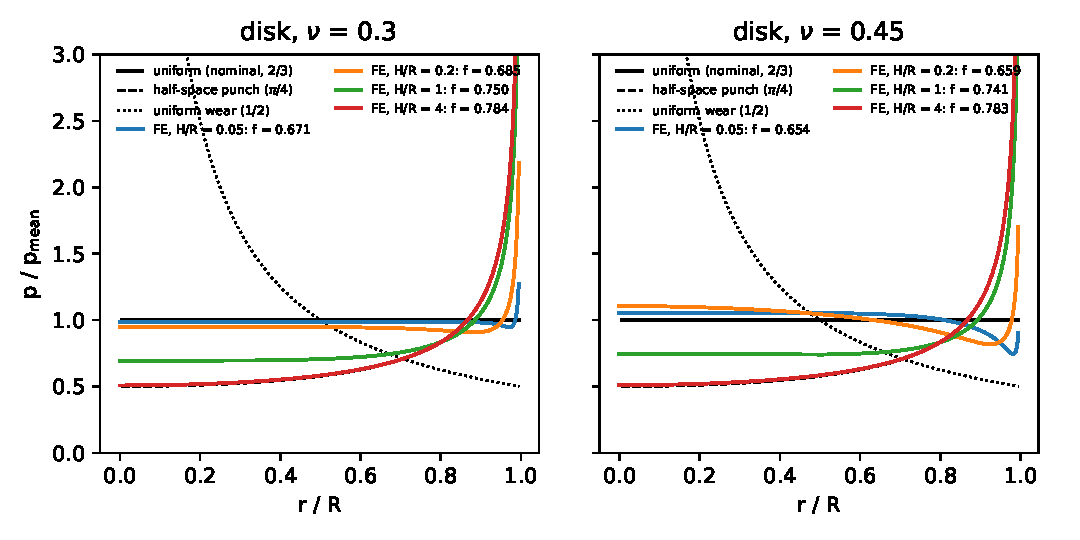
\includegraphics[width=0.9\linewidth]{../results/fem/figures/disk_pressure.pdf}\\[2pt]
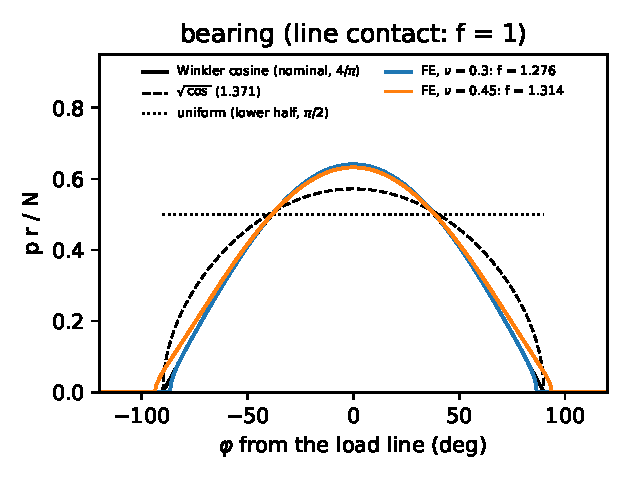
\includegraphics[width=0.55\linewidth]{../results/fem/figures/bearing_pressure.pdf}
\caption{Pressure of a linear-elastic support computed by finite elements (Section~5.4 of the
paper) against the distributions of the band. Top: \scn{disk}, layers of several thicknesses
$H/R$ under a rigid flat punch, for $\nu=0.3$ and $0.45$. Bottom: \scn{bearing}, plane-strain
sleeve around a rigid journal}
\label{sup:fem}
\end{figure}

\subsection{The friction quadratures on the battery}

Table~\ref{tab:ablation} compares \law{distributed} with its two quadrature variants and with
\law{pcm} on the meshes of the battery. In \scn{contensou} the closed form has
\result{err/contensou/distributed} against \result{err/contensou/vertex} and
\result{err/contensou/centroid}. In \scn{ring}, whose centre of rotation is outside the face,
the battery's own triangulation already gives \result{tri/ring/spin/quads/64/centroid/moment}
and \result{tri/ring/spin/quads/64/vertex/moment} in the experiment on one face, and the three
rules agree in the battery. Over class A the ratio of the errors of \law{distributed} to those
of its vertex variant is \result{robust/distributed-vs-vertex/A/full} with
\result{robust/distributed-vs-vertex/A/ties} ties in \result{robust/distributed-vs-vertex/A/n}
units, the one unit that differs being the cut ground. The battery's errors are stop times and
combine the two sides of the contact, so they are not the torque errors of the experiment on
one face (\code{tools/ablation\_triangulation.py}). The cost of a quadrature on a remeshed face
at equal accuracy, through the geometry of the larger number of polygons, was not measured.
\law{pcm}, even with the exact contact surface lent to it, has the error of its one-point
friction on the battery's spinning flat contacts and depends on the cut, both of which a finer
mesh of the flat faces would reduce; it cannot hold a body still (\scn{push}, \scn{wedge},
\scn{tip}, \scn{stack}, \scn{tower}), which no mesh changes; and it is the better of the two on
curved conforming contact (\result{err/bearing/pcm} against \result{err/bearing/distributed} in
\scn{bearing}, \result{err/journal/pcm} against \result{err/journal/distributed} in
\scn{journal}).

\begin{table}[!htbp]
\caption{The battery, on its own meshes (flat caps: fans from a rim vertex; grounds: two
triangles per face): error [\%] of the distributed law with the closed-form friction, with the
vertex rule and with the one-point rule, and of the per-face foundation, on the flat spinning
contacts under refinement of the curved meshes (1\,ms) and on the ground cut into pieces}
\label{tab:ablation}
\generatedtable{ablation}
\end{table}

\subsection{Convergence with the step and the mesh}

Table~\ref{tab:convergence} classifies every series by the slope of the logarithm of the error
against the logarithm of the step or of the mesh size as converging, flat (a slope within
$\pm0.2$, or every error below $2\times10^{-3}$), diverging, non-monotone or failed.
Figures~\ref{fig:convergence-dt} and~\ref{fig:convergence-mesh} show the error against the step
and the number of segments in selected scenarios. A flat step series is evidence about the law
as given only where the step bounds of Section~\ref{sup:bounds} are inactive; where they act
(\scn{tower}, \scn{massratio}, \scn{stack}), the applied parameters change with the step.

\begin{table}[!htbp]
\caption{Convergence series by method: number of scenarios in which the error converges
(conv.), stays flat, is not monotone (n-m.), diverges (div.) or a run of the series did not
finish (fail.), with the step (2 to 0.1\,ms) and with the mesh (32 to 128 segments)}
\label{tab:convergence}
\generatedtable{convergence}
\end{table}

\begin{figure}[!htbp]
\centering
\generatedfigure{convergence_dt}
\caption{Error [\%] against the time step in six scenarios. Errors above 3000\,\% are drawn at
that value; a missing point is a run without an error value. Chrono SMC is not shown: its
backend sub-steps}
\label{fig:convergence-dt}
\end{figure}

\begin{figure}[!htbp]
\centering
\generatedfigure{convergence_mesh}
\caption{Error [\%] against the number of segments per turn of the curved meshes in six
scenarios, at 1\,ms}
\label{fig:convergence-mesh}
\end{figure}

\subsection{The stiffness series and the energy measure}

Table~\ref{tab:stiffness} and Fig.~\ref{fig:stiffness} show the effect of a tenfold stiffer
foundation. On class A the error of \law{distributed} falls in \scn{edge}
(\result{err/edge/distributed/dt0.2} to \result{err/edge/distributed/stiff}), \scn{turntable},
\scn{bowl}, \scn{trough}, \scn{billiard}, \scn{oblique} and \scn{journal}, and rises in
\scn{cylinder} and in \scn{massratio}. On the flat \scn{disk} the errors of the two laws rise
(\law{gonthier}: \result{err/disk/gonthier/stiff}) and those of Drake hydroelastic and
\law{pcm} do not (\result{err/disk/hydro/stiff}, \result{err/disk/pcm/stiff}); in the
diagnostic runs behind the flutter condition of the paper the rocking and vertical modes had
$K\,w\,\dt^2$ of 0.08 at 0.2\,ms, and the tilt saturated at about 65 times its amplitude at
$K$. In the diagnostic run of \scn{cone} at $10K$ the frustum wobbled by 0.065\,rad and climbed
out of its seat, at an error that did not depend on the step.
% Diagnostic single runs on Chrono, docs/research/anomalies.md §1.

\emph{The energy measure.} Over the perturbed starts the measure of \scn{energy} covers
\result{pertrange/energy/gonthier/range} for \law{gonthier},
\result{pertrange/energy/pcm/range} for \law{pcm} and
\result{pertrange/energy/distributed/range} for \law{distributed}. For \law{gonthier} it falls
to \result{err/energy/gonthier/mesh128} with 128 segments, and in diagnostic runs at the base
step with ten times the stiffness, where the penetration and the energy that it stores are
smaller, it was 0.02 to 0.03\,\% for the two laws; in the diagnostic run at the base stiffness
the energy never exceeded its start by more than 1.8\,\%.
% 0.016 %, 0.03 % and 1.8 %: single diagnostic runs, docs/research/anomalies.md §2
The single run made when the scenario was written gave \result{first/energy/gonthier} for
\law{gonthier}; since the runs are deterministic, something changed the nominal trajectory
between that commit and the battery, and which change it was has not been identified (it was
not bisected).

\begin{table}[!htbp]
\caption{Error [\%] at the stiffness of the scenario and at ten times that stiffness
($K \to 10K$), both at 0.2\,ms, classes A and B}
\label{tab:stiffness}
\generatedtable{stiffness}
\end{table}

\begin{figure}[!htbp]
\centering
\generatedfigure{stiffness}
\caption{Error [\%] of the distributed law and of Drake hydroelastic at the stiffness of each
scenario and at ten times that stiffness, at 0.2\,ms. The dotted line separates class A from
class B; a cross is a run without an error value}
\label{fig:stiffness}
\end{figure}

\subsection{Cost}\label{sup:cost}

Table~\ref{tab:cost} gives the cost of every method and Fig.~\ref{fig:work-precision} sets it
against the share of scenarios solved within 5\,\%. The timings are those of
\result{cost/source}, with the code of commit \result{battery/timing-commit} on
\result{battery/timing-date}; the two friction quadratures were not timed, and Chrono SMC is
sub-stepped by its backend. Drake hydroelastic did not finish \scn{tower} within the limit of
the timing pass, so \scn{tower} is not in its median or its maximum. The only figure for that
run is of another kind and is not comparable with the timings: in the accuracy pass, on a
loaded machine, it used its hour of time limit without finishing, which puts its cost above
\result{cost/bound/tower-hydro} times real time, a lower bound that the load inflates by an
unknown factor. The costs of the native models are those of our configurations at the step of
the battery, not at the larger steps that implicit solvers allow.

\begin{table}[!htbp]
\caption{Wall-clock time over simulated time across the scenarios, base variant
(\result{cost/label}). Runs: scenarios timed; Drake hydroelastic did not finish \scn{tower}}
\label{tab:cost}
\generatedtable{cost}
\end{table}

\begin{figure}[!htbp]
\centering
\generatedfigure{work_precision}
\caption{Share of class A and B scenarios within 5\,\% against the wall-clock time over the
simulated time (\result{cost/label}). Marker: median over the scenarios; bar: 10th to 90th
percentile}
\label{fig:work-precision}
\end{figure}

\clearpage
\section{Statistical inference and sensitivity}\label{sup:inference}

% The paper cites these subsections by number (S5.1 to S5.5): keep their order.

The paper reports one paragraph and one table of paired comparisons (its Section~5.10). This
section gives the rules behind them, every pair, and how the figures move when the rules
change. The scenarios were chosen by hand, several test the same mechanism (five are the
friction torque of a spinning conforming contact, three a body rolling against the foundation's
rolling resistance) and class B has five, so the bootstrap treats as exchangeable units that are
not: the intervals and the $p$-values are descriptive.

\subsection{Rules}

All summaries use the base variant. For two methods on the same scenarios we report the
geometric mean of the ratio of their errors with a 95\,\% percentile interval from 10\,000
bootstrap resamples within class, under the following rules.
\begin{itemize}
\item \emph{Cap and failures.} An error above \result{rules/cap} counts as \result{rules/cap},
  and so does a run without an error value, for whichever method it belongs to. No scenario is
  left out. Errors below \result{rules/floor} count as \result{rules/floor}. Without the cap, a
  run that ends with an enormous error (the two laws in \scn{massratio}, where the bodies fly
  apart) weighs several decades, by an amount that is arbitrary, while a run that fails without
  a value weighs nothing.
\item \emph{Clusters.} The four \scn{pieces} scenarios are the same problem on four cuts of
  the ground; they enter once, with the mean of their logarithmic ratios.
\item \emph{Ties.} A scenario is won or lost only if the two errors differ by more than a
  factor of \result{rules/tie}; otherwise it is a tie.
\item \emph{Leave-one-out.} Every ratio is given with the range that it covers when one
  unit is removed.
\item \emph{Primary comparisons and multiplicity.} \result{primary/n} comparisons are tested:
  \law{distributed} against \law{gonthier}, and each of the two against the default native
  model of each engine in this paper (Drake hydroelastic, Chrono SMC, MuJoCo soft), on class A
  and on classes A and B. Their bootstrap $p$-values, computed from the bootstrap distribution
  itself and not from a sample of it, are adjusted with Holm's method over that family, and
  ``significant'' means an adjusted $p$ below 0.05. Every other pair is exploratory and is
  reported without a test.
\end{itemize}
The cap, the tie band and the family were fixed after the data had been seen: the family is a
reduction of the number of tests, not a pre-registration. A law is compared with a native model
on that model's engine.

\subsection{Primary comparisons}

Table~\ref{tab:ratios} gives the primary comparisons with their leave-one-out ranges and their
counts of units won, tied and lost, next to the uncapped estimate, and Fig.~\ref{fig:forest}
their intervals. Of the \result{primary/n}, \result{primary/significant} are significant after
Holm's correction, both on classes A and B together: \law{distributed} against \law{gonthier}
(\result{robust/distributed-vs-gonthier/A+B/full}, adjusted $p = $
\result{robust/distributed-vs-gonthier/A+B/holm}) and against Chrono SMC
(\result{robust/distributed-vs-smc/A+B/full}, adjusted $p = $
\result{robust/distributed-vs-smc/A+B/holm}, close to the threshold). Two more have an
unadjusted interval that excludes 1 and do not survive the correction: \law{distributed}
against Drake hydroelastic (\result{robust/distributed-vs-hydro/A+B/full}) and against MuJoCo
soft (\result{robust/distributed-vs-soft/A+B/full}). On class A alone
\result{primary/significant/A} of the \result{primary/n/A} comparisons is significant: the two
laws are not separated from each other (\result{robust/distributed-vs-gonthier/A/full}, with
\result{robust/distributed-vs-gonthier/A/ties} ties in
\result{robust/distributed-vs-gonthier/A/n}), and against the default native models their
ratios are below 1 with intervals that reach above it (\law{distributed}:
\result{robust/distributed-vs-hydro/A/full} against Drake hydroelastic,
\result{robust/distributed-vs-smc/A/full} against Chrono SMC,
\result{robust/distributed-vs-soft/A/full} against MuJoCo soft). The count of scenarios says
more than the mean there: \law{distributed} has the smaller error by more than the tie band in
\result{robust/distributed-vs-hydro/A/wins}, \result{robust/distributed-vs-smc/A/wins} and
\result{robust/distributed-vs-soft/A/wins} of the \result{robust/distributed-vs-hydro/A/n}
units (won, tied and lost: \result{robust/distributed-vs-hydro/A/wtl},
\result{robust/distributed-vs-smc/A/wtl} and \result{robust/distributed-vs-soft/A/wtl}), and the
scenarios that it loses, it loses by much (\scn{massratio} against the two implicit solvers,
the sliding and rolling scenarios where a penalty or constraint model is at the floor).

\begin{table}[!htbp]
\caption{Primary comparisons: ratio of the errors of two methods on the same scenarios, base
variant. Reported: errors capped at \result{rules/cap}, runs without a value counted at the
cap, the \scn{pieces} scenarios one unit; $p$: bootstrap, Holm-adjusted over the
\result{primary/n} comparisons (bold: below 0.05); leave-one-out: range of the ratio when one
unit is removed; W/T/L: units won, tied (ratio within \result{rules/tie}) and lost by the first
method. Uncapped: raw errors, scenarios that a method did not finish left out (their number in
brackets), every scenario one unit}
\label{tab:ratios}
\generatedtable{ratios_primary}
\end{table}

\begin{figure}[!htbp]
\centering
\generatedfigure{forest_primary}
\caption{The primary comparisons with their 95\,\% bootstrap intervals, as reported and
uncapped}
\label{fig:forest}
\end{figure}

\subsection{Exploratory comparisons}

Table~\ref{tab:ratios-robust} gives every pair under the same rules, with unadjusted intervals
and no test. On class A \law{distributed} is not separated from Drake point
(\result{robust/distributed-vs-dpoint/A/full}) or from Chrono NSC
(\result{robust/distributed-vs-nsc/A/full}); on classes A and B its ratios to Drake point, to
Chrono NSC and to MuJoCo default are \result{robust/distributed-vs-dpoint/A+B/full},
\result{robust/distributed-vs-nsc/A+B/full} and
\result{robust/distributed-vs-mjdefault/A+B/full}. The error of \law{gonthier-thesis} is
\result{robust/thesis-vs-gonthier/A/full} times that of \law{gonthier} on class A: the friction
that Gonthier published, with the bristle on the material slip, is several times more accurate
than the variant of the 2018 thesis, which loses the scenarios in which a body must be held.
The error of \law{distributed} is \result{robust/distributed-vs-pcm/A+B/full} times that of
\law{pcm}.

\begin{table}[!htbp]
\caption{Every pair under the rules of the primary comparisons: geometric mean of the ratio of
the capped errors, 95\,\% bootstrap interval (unadjusted), and units won, tied and lost by the
first method}
\label{tab:ratios-robust}
\generatedtable{ratios_robust}
\end{table}

\subsection{Sensitivity analyses}

\emph{Without the cap.} Table~\ref{tab:ratios-first} gives the same pairs on the raw errors,
with the scenarios that either method did not finish left out and every scenario one unit; no
conclusion rests on it. On that estimate no interval of a law against a native model on class A
excludes 1, and the intervals span one to two orders of magnitude: \scn{massratio} enters with
the nearly seven decades between the error of a lost run and the floor, while the runs that the
native models did not finish are left out. Capping the errors and counting the failures moves
every primary ratio of a law against a native model towards the laws (on class A, from between
\result{ratio/distributed-vs-hydro/A/gm} and \result{ratio/gonthier-vs-soft/A/gm} to between
\result{robust/distributed-vs-hydro/A/gm} and \result{robust/gonthier-vs-soft/A/gm}) and
narrows the intervals; the choice of rules therefore favours the laws. For \law{gonthier-thesis} against
\law{gonthier} the uncapped ratio on class A is \result{ratio/thesis-vs-gonthier/A/full}.

\emph{Leave-one-out.} Removing any one unit leaves every primary ratio of a law against a
native model below or at 1 (Table~\ref{tab:ratios}).

\emph{Reduced class A.} Table~\ref{tab:reduced} repeats the primary comparisons on class A
without \scn{bowl}, \scn{trough}, \scn{turntable} and \scn{edge}, whose references no damped
compliant model can meet at the $h$ and $K$ of the battery: the ratios move by less than their
intervals, and none excludes 1. The counts within 5\,\% on the reduced class are
\result{pass/Ar/distributed/5} for \law{distributed}, \result{pass/Ar/gonthier/5} for
\law{gonthier}, and between \result{passn/Ar/mjdefault/5} and \result{passn/Ar/hydro/5} for the
native models (on the whole class A, \result{pass/A/distributed/5},
\result{pass/A/gonthier/5}, and between \result{passn/A/mjdefault/5} and
\result{passn/A/hydro/5}; within 1\,\%, \result{passn/A/distributed/1} for \law{distributed}
and \result{passn/A/dpoint/1} for Drake point; on class B within 5\,\%,
\result{pass/B/distributed/5} for \law{distributed}, \result{pass/B/hydro/5} for Drake
hydroelastic, \result{pass/B/gonthier/5} for \law{gonthier} and at most
\result{passn/B/smc/5} for a point-contact model).

\emph{Perturbed starts.} Over the eight perturbations of the initial velocities the range of
the error relative to its median has a median over the scenarios of \result{pert/gonthier} for
\law{gonthier} and \result{pert/distributed} for \law{distributed}: the base errors of the laws
are representative of nearby initial conditions. Those of several native models are not
(Section~\ref{sup:scatter}), so for them single base runs enter the ratios as draws.

\begin{table}[!htbp]
\caption{Uncapped estimate: ratio of the raw errors of two methods on the same scenarios, base
variant: geometric mean, 95\,\% bootstrap interval, and scenarios won and lost by the first
method (in brackets, the scenarios left out because one of the two did not finish). Bold: the
unadjusted interval excludes 1}
\label{tab:ratios-first}
\generatedtable{ratios}
\end{table}

\begin{table}[!htbp]
\caption{The primary comparisons on class A and on class A without the four parameter-bound
scenarios}
\label{tab:reduced}
\generatedtable{reduced}
\end{table}

\subsection{Runs that would settle the open points}

The following would answer open points of the paper and were not done. (1) Log, for every run,
whether the step bounds were active and the extreme ratios of the applied to the nominal
parameters ($h$, $d$, $v_s$, stick stiffness). (2) Record the sign of the class B errors, to
place every run against the band (the paper's Section~5.4 signs those of \scn{disk} and
\scn{bearing} only). (3) One more decade of stiffness ($K\times100$) on class A,
at the step that the laws need. (4) \scn{journal} at 256 segments with the climb angle
reported, and \scn{cone} at $10K$ with 128 segments, to separate the facet sag from the
self-excited wobble. (5) Sweeps of $d$ and $\tau$ on the scenarios that hold a body
(\scn{push}, \scn{wedge}, \scn{tower}, \scn{stack}, \scn{tip}, \scn{hole}), and of $h$ on the
rolling ones. (6) Native models again with reviewed configurations: Drake point with rim
spheres on cylinder faces, MuJoCo soft on \scn{block}, repeated or better converged runs of
Chrono NSC, and a check of the static penetration of every native model per scenario. (7) A
bisection of the change of \law{gonthier} in \scn{energy} between the first run of the second
set and the battery, and an energy measure that counts the contact spring. (8) The linear
stability model with the discrete sums of \law{pcm}, to explain why it does not flutter. (9)
The quadratures on remeshed flat faces inside the library, with their cost at equal accuracy.
(10) Finite-element solutions for the other class B scenarios (\scn{ring}, \scn{contensou},
\scn{cone}; the paper's Section~5.4 covers \scn{disk} and \scn{bearing}, statically), a
dynamic one with friction, measured data for one class B case, and three to five scenarios
written and frozen before any run, as a true out-of-sample check.

\clearpage

\bibliography{references}

\end{document}
